
\documentclass{beamer}

%\usetheme{Malmoe}
%\usetheme{Luebeck}
\usetheme{Darmstadt}
\usecolortheme{rose}
\usepackage[latin1]{inputenc}

\title{Intro to Linux}
\author{Stephen Wattam}
\date{October 11th, 2010}
\institute[2010]{Computing Society of Lancaster University}

\begin{document}

\frame{\titlepage}

\section[Outline]{}
\frame{\tableofcontents}
\frame{ \frametitle{How we do this}

    \begin{center}How much experience do people have?\end{center}
    \vspace{10pt}


    \begin{block}{}
	\begin{enumerate}
\vspace{7pt}
		\item<1-> What is this linux thing you speak of?
\vspace{7pt}
		\item<2-> I aim to use Linux day-to-day.
\vspace{7pt}
		\item<3-> I want to code and understand stuff!
\vspace{7pt}
		\item<4-> SHOW ME THE KERNEL SOURCE!!!!!1.
\vspace{7pt}
	\end{enumerate}
    \end{block}
}




\section{Operating Systems}
\subsection{Parts of OSs, Hardware}
\frame{ \frametitle{Basic OS Components}
    \begin{itemize}
	\item Kernel (drives the hardware)
	\item User-Space (where your programs reside)
	\item Operating environment (shell)
	\item Programs and Libraries
    \end{itemize}

    \begin{figure}
	\scalebox{0.27}{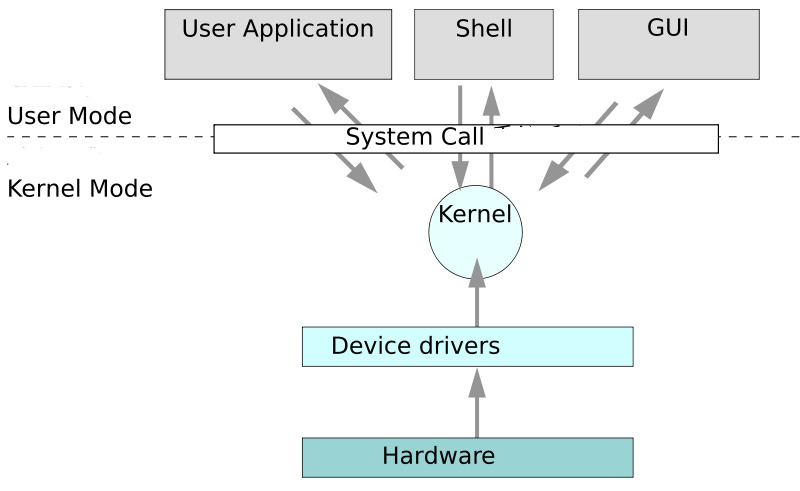
\includegraphics{images/osdiagram.png}}
    \end{figure}



}

% install both on one system, partitions
\subsection{Running Software}
\frame{ \frametitle{The OS Controls...}
    \begin{itemize}
	\item Loading programs into RAM
\vspace{7pt}
	\item Controlling many programs at once
\vspace{7pt}
	\item Managing hardware devices
\vspace{7pt}
	\item Managing libraries used by those programs
    \end{itemize}
}

% ELF vs exe



\section{History}
\subsection{The Early Years}
\frame{ \frametitle{Mainframes}
    \begin{itemize}
	\item Machines mainly used for large business/research
	\item Many users to a machine (time-sharing)
	\item Teletypes!
	\item `Vast' data storage, commonly on tape
	\item Operating as a service
	\item OS: VAX, UNIX etc
    \end{itemize}

    \begin{figure}
	\scalebox{0.27}{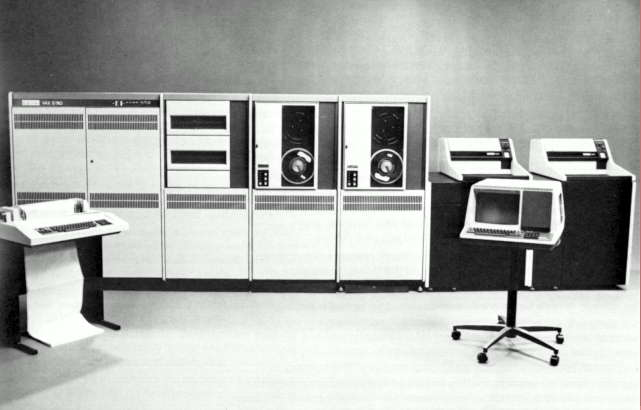
\includegraphics{images/vax11.jpg}}
    \end{figure}
}
% mainframes, lisp, early home systems
\subsection{The Rise of the PC}
\frame{ \frametitle{Personal Computers}
    \begin{itemize}
	\item Smaller and simpler machines for smaller tasks
	\item One user to a machine
	\item Used from the same machine
	\item Memory was very expensive, very little storage
	\item Operating as an Appliance
	\item OS: DOS, ACORN, Apple OS
    \end{itemize}
    
    \begin{figure}
	\scalebox{0.27}{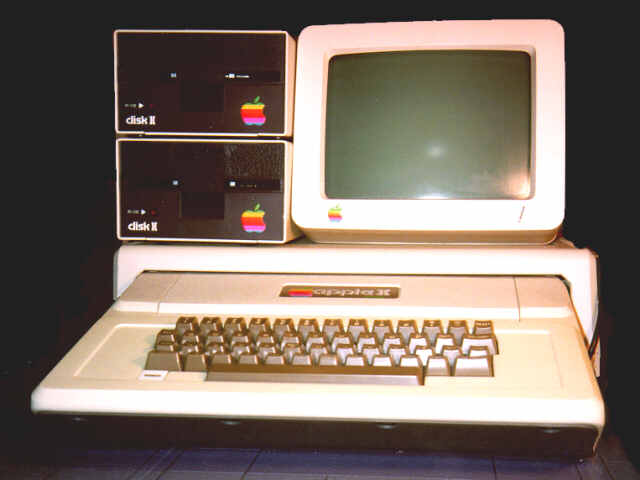
\includegraphics{images/Apple2Plus.jpg}}
    \end{figure}
}
% BeOS, amiga, DOS, win3.1
\subsection{The NeXT STEP}
\frame{ \frametitle{Ubiquity}
    \begin{itemize}
	\item The PC became more capable
	\item Multiple people (families) to a machine
	\item Mega storage through technical advances
	\item Moving back to client/server, slightly.
	\item OS: Windows 9x/XP, OSX, Linux, OS/2
    \end{itemize}

    \begin{figure}
	\scalebox{0.27}{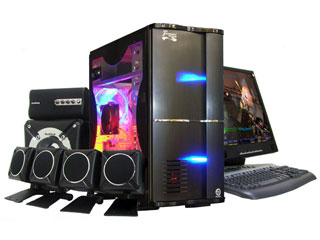
\includegraphics{images/custompc.jpg}}
    \end{figure}

}
% Apple and BSD, unix links
\subsection{Linux in Context}
\frame{ \frametitle{Development of Linux}
    \begin{itemize}
	\item Developed by Linus Torvalds from Minix
	\item Gradual interest from early 90's
	\item Tied to GNU project from Stallman
	\item Gained popularity on servers
	\item Found to be a decent desktop OS too
    \end{itemize}


    \begin{figure}
	\scalebox{0.57}{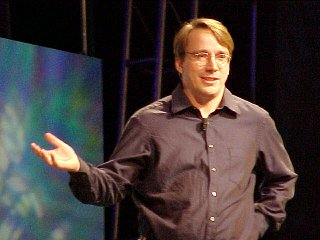
\includegraphics{images/linus.jpg}}
    \end{figure}
}
% Minix, Linus Torvalds, GNU



\section{Linux vs. Windows vs. Mac OSX}
\subsection{Centralised vs. Decentralised}
\frame{ \frametitle{Commercial Interests}


    \begin{columns}[c]
    \column{2.0in}


	\begin{block}{Linux}
	    \begin{itemize}
		    \item<1-> Very flexible --- comprised of many projects
		    \item<2-> Open --- All source code is editable
		    \item<3-> Progress defined purely by market forces
		    \item<4-> Focus on improving software for own use
	    \end{itemize}
	\end{block}


    \column{2.0in}
    
	\begin{block}{Mac/Win}
	    \begin{itemize}
		    \item<1-> Available only as a pre-rolled package
		    \item<2-> Closed --- Source is closely guarded
		    \item<3-> Progress defined by one coherent vision
		    \item<4-> Focus on shipping features to customers
	    \end{itemize}
	\end{block}
    
    \end{columns}


}



\subsection{DLLs vs Deps}
\frame{ \frametitle{Centralised Architecture}
    \begin{itemize}
	\item Windows, in the 90's, chose central control
\vspace{7pt}
	\item Windows registry, DLLs, DCOM, service APIs
\vspace{7pt}
	\item These have not scaled well now that PCs are very 'large'
\vspace{7pt}
	\item The unix philosophy was designed for large machines, and has weathered better
    \end{itemize}
}

\subsection{Unix Philosophy}
\frame{ \frametitle{The UNIX Philosophy}
    \begin{itemize}
	\item Everything is a file (and can be controlled through read/write calls)
\vspace{7pt}
	\item Tools should do one thing, and do it well
\vspace{7pt}
	\item Tools should accept text in, and output text (as a universal interface)
	% more?
    \end{itemize}
}


% windows, linux, mac


\section{Overview}
\subsection{File System}
\frame{ \frametitle{File System Structure}
    \begin{itemize}
	\item One root directory, \texttt{/}
	\item Home directories all stored together, \texttt{/home/username/}
	\item Configuration stored in \texttt{/etc/}
	\item Programs stored in \texttt{/bin/}
	\item User-installed (non-system) programs at \texttt{/usr/bin/}
    \end{itemize}
}
\frame{ \frametitle{File System Structure}
    \begin{figure}
	\scalebox{1.4}{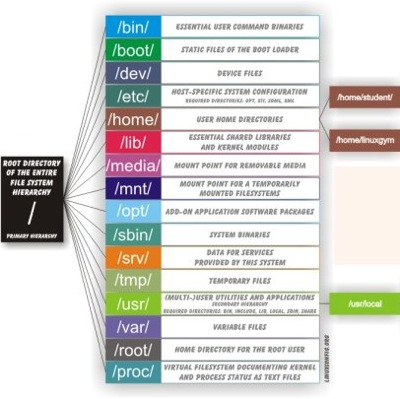
\includegraphics{images/unixfsh.jpg}}
    \end{figure}
}

\subsection{CLI vs Graphical}
\frame{ \frametitle{The command line}
    \begin{itemize}
	\item Linux (and other unices) retain their TTy support
	\item Command lines are emulators for TTy hardware
	\item The linux/unix command line is very well developed
	\item Because of the unix philosophy, almost everything can be done through the command line
    \end{itemize}


    \begin{figure}
	\scalebox{0.3}{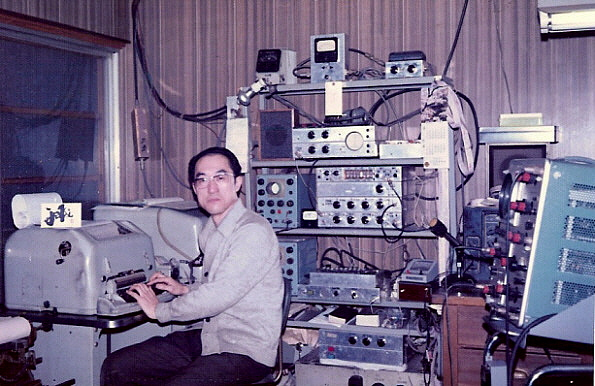
\includegraphics{images/tty.jpg}}
    \end{figure}
}
\subsection{Shells}
\frame{ \frametitle{Graphical Shells}
    \begin{itemize}
	\item Normally \texttt{explorer.exe} in Windows
	\item In Linux, we run a program on top of the CLI to provide graphical output
	\item The only widely used one is called X, and uses the X11 protocol
	\item This protocol gives us some cool features for free
    \end{itemize}

    \begin{figure}
	\scalebox{0.3}{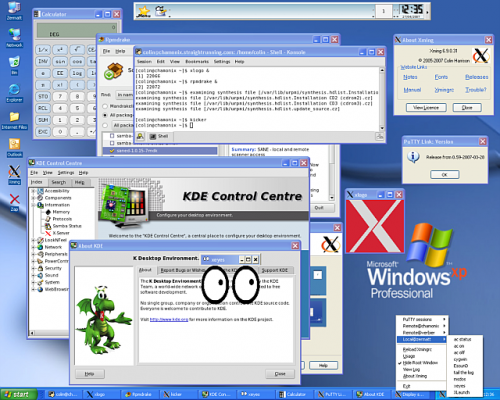
\includegraphics{images/xinwin.png}}
    \end{figure}

}
\subsection{Window Managers}
\frame{ \frametitle{Window Managers}
    \begin{itemize}
	\item X provides an API to manage windows and rendering
	\item But it does not tell people how to display them
	\item A window manager does all organisation and display
	\item There are hundreds to choose from, and they all work in different ways
	\item Pick one to suit
    \end{itemizeo}


    \begin{figure}
	\scalebox{0.15}{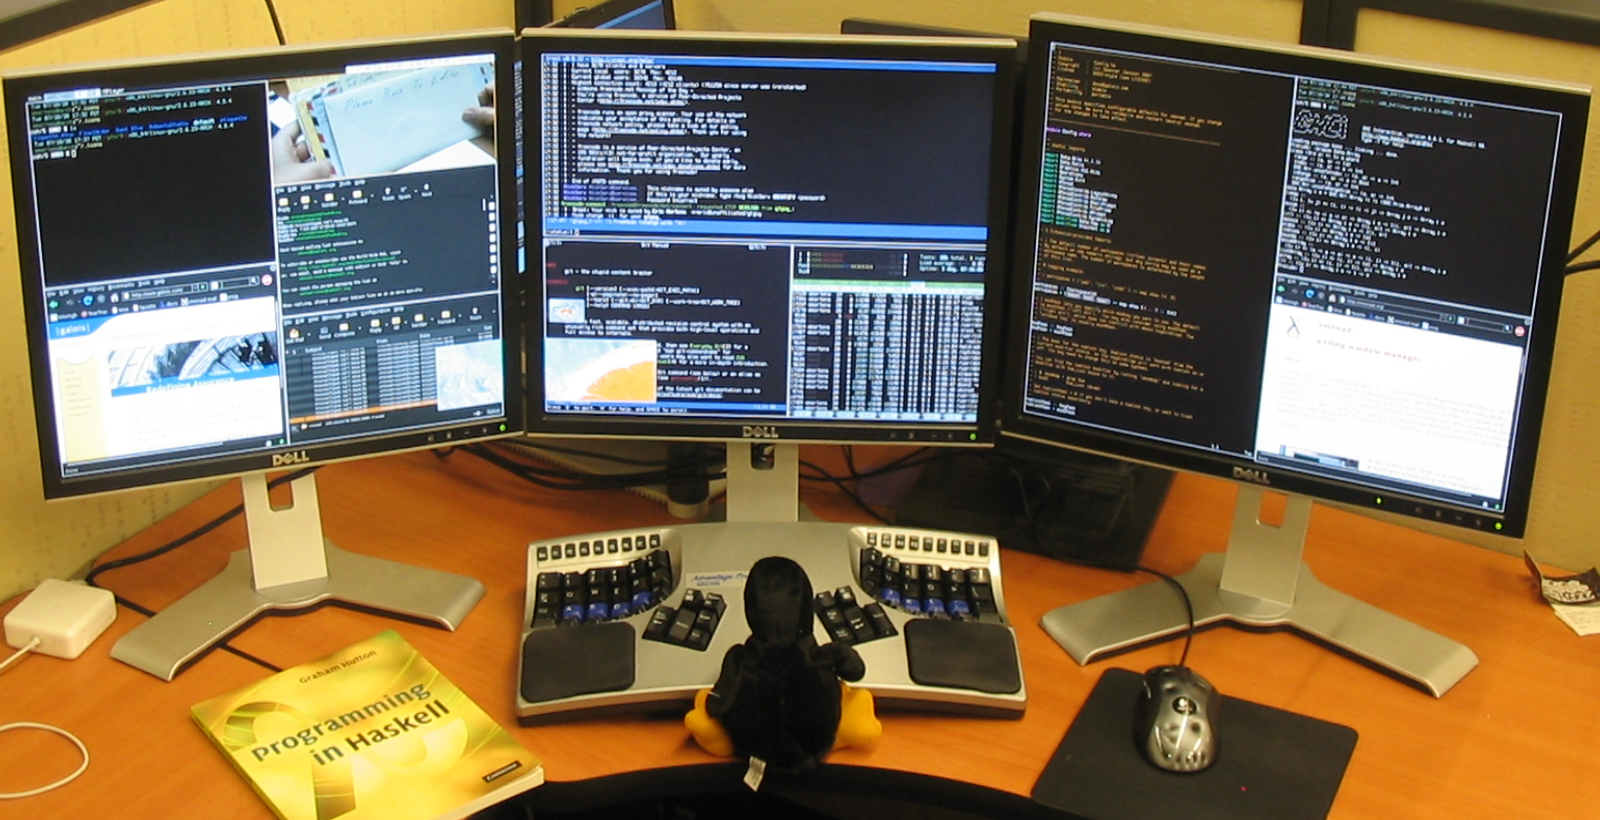
\includegraphics{images/xmonad.png}}
    \end{figure}
}



\section{Nerding out}
\subsection{Command Line Productivity}
\frame{ \frametitle{Shell Scripting}
    \begin{itemize}
	\item Simple tools may be combined in interesting ways
\vspace{7pt}
	\item Files may be redirected as input and/or output
\vspace{7pt}
	\item FIFOs, links and sockets may be used to emulate other parts of the system
\vspace{24pt}
	\item \texttt{ \$ grep 'Title' spells.txt | sort | uniq -c | sort -n -r | head -10 > popular\_spells.txt }
    \end{itemize}

}
\subsection{Well-designed applications}
\frame{ \frametitle{Application Design}
    \begin{itemize}
	\item Applications managed by dedicated teams
	\item Code quality boosted by the hobby approach
	\item Text in, Text out
	\item Simple, standard, tools mean they may be used in programs
	\item Decades old programs like vim and emacs are best-in-class
    \end{itemize}

    \begin{figure}
	\scalebox{0.15}{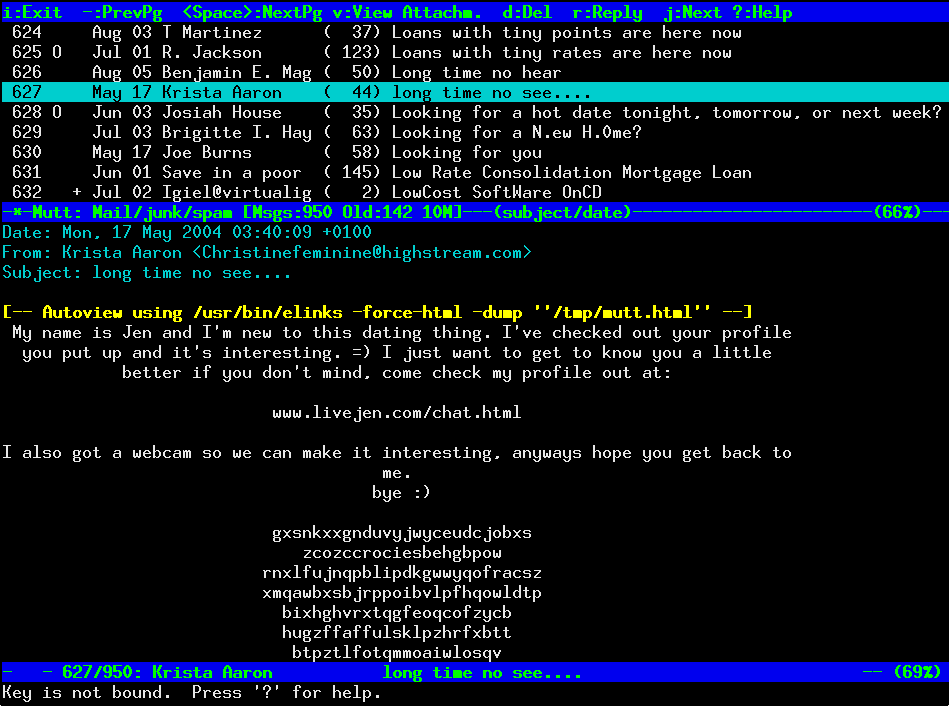
\includegraphics{images/mutt.png}}
    \end{figure}

}
\subsection{Unique Unix Abilities}
\frame{ \frametitle{Unix Heritage}
    \begin{itemize}
	\item Robust security systems are well proven
\vspace{7pt}
	\item Scaleability and flexibility have been maximised
\vspace{7pt}
	\item Everything-is-a-file is very handy
\vspace{7pt}
	\item Network transparent usage (from original time-sharing designs)
\vspace{7pt}
	\item Many systems, such as the internet, were designed on and for unix
\vspace{7pt}
    \end{itemize}
}
% pipes, block devices, everything is a file

\section{Demo}
\frame{ \frametitle{Demo}
}

%% -----------------------------------------------------------------------------------------
%\section{Constitution}

%\subsection{Remit}
%\frame{ \frametitle{Why have a Computing Society?}

    %\begin{center}We are primarily an \textsl{academic} society:\end{center}
    %\vspace{10pt}


    %\begin{block}{From the Constitution}
	%\begin{itemize}
		%\item<1-> Provide an opportunity to all those interested in ``Computers and Computing" to get together.
		%\item<2-> Give a general understanding of programming.
		%\item<3-> Look into computer hardware and uses.
		%\item<4-> Open up research ideas.
		%\item<5-> In some cases could help to get contacts within industry.
	%\end{itemize}
    %\end{block}
%}


%\subsection{Membership}
%\frame{ \frametitle{Membership Status}

    %\begin{center}Full, Honorary, and Associate Members\end{center}
    %\vspace{10pt}


    %\begin{columns}[c]
    %\column{2.0in}


	%\begin{block}{Full Members}
	    %\begin{itemize}
		    %\item<1-> Can Propose Motions during meetings
		    %\item<2-> Must attend GMs
		    %\item<3-> Can vote/nominate candidates for the exec
		    %\item<4-> Must be paid/registered with LUSU
	    %\end{itemize}
	%\end{block}


    %\column{2.0in}
    
	%\begin{block}{Associate Members}
	    %\begin{itemize}
		    %\item<5-> Not well defined in the Constitution
		    %\item<6-> May attend, speak at meetings
		    %\item<7-> May not vote or nominate in GMs, but may attend
		    %\item<8-> Unclear LUSU Status
	    %\end{itemize}
	%\end{block}
    
    %\end{columns}



    

%}

%\subsection{Exec Committee}
%\frame{ \frametitle{Exec Roles}

    %\begin{center}
	%The CS Exec contains the following roles:

    %\begin{itemize}
	    %\item<1-> President (Carl)
    %\vspace{7pt}
	    %\item<2-> Secretary (Steve)
    %\vspace{7pt}
	    %\item<3-> Treasurer (Jasmine)
    %\vspace{7pt}
	    %\item<4-> Social Sec. (Dan/Ron)
    %\vspace{7pt}
	    %\item<5-> Vice President (Chris)
    %\vspace{7pt}
	    %\item<6-> Publicity (Matt)
    %\vspace{7pt}
	    %\item<7-> Webmaster (Pjotr)
    %\end{itemize}
    
    %\end{center}
%}


%\frame{ \frametitle{Exec Rules}
    %\begin{itemize}
	%\item<1-> Attendance at GMs is mandatory on condition of expulsion (apologies may be sent in writing)
    %\vspace{7pt}
	%\item<2-> Office runs from last day of lent term for one year
    %\vspace{7pt}
	%\item<3-> Incompetence may result in suspension/motion of no confidence
    %\vspace{7pt}
	%\item<4-> Meetings with the exec at [Time, place TBA]
    %\end{itemize}

%}



%\subsection{Elections}
%\frame{ \frametitle{Election Process}
    %\begin{itemize}
	%\item<1-> Elections for all Officers at AGM, Lent term
    %\vspace{7pt}
	%\item<2-> By-elections may be called in any other GM (next week)
    %\vspace{7pt}
	%\item<3-> Elections are based on a short presentation of some form, then questions
    %\vspace{7pt}
	%\item<4-> RON is always a candidate
    %\vspace{7pt}
	%\item<5-> Candidates must submit written intent to stand
    %\end{itemize}
%}


%\subsection{General Meetings}
%\frame{ \frametitle{GM}
    %\begin{itemize}
	%\item<1-> Three a year, at least
    %\vspace{7pt}
	%\item<2-> AGM is in the 'last few weeks' of lent term
    %\vspace{7pt}
	%\item<3-> Quorum conditions (max):
	%\begin{enumerate}
		%\item Ten full members.
		%\item At least 15\% of the Society membership.
		%\item 150\% of the Society Executive Committee -- This is the Society Executive Committee plus 50\% of the size of the Society Executive Committee in non-Society Executive Committee members.
	%\end{enumerate}
    %\end{itemize}
%}



%\section{Next Week's Meeting}

%\subsection{About the Meeting}

%\frame{ \frametitle{GM Status}
    
    %\begin{itemize}
	%\item<1-> We need two weeks' notice to call a 'full GM'
    %\vspace{7pt}
	%\item<2-> Since we had no members two weeks ago, this was particluarly easy ;-)
    %\vspace{7pt}
	%\item<3-> We can thus avoid calling a second GM later this term
    %\end{itemize}
%}


%\subsection{Agenda}
%\frame{ \frametitle{Agenda - Social Sec}
    %\begin{center}We need a Social Secretary\end{center}

    %\begin{block}{From the Constitution}
	%\begin{itemize}
	    %\item Organise and publicise a wide range of social events and activities for all members.
	    %\item Ensure that the safety aspects of such activities are satisfactorily addressed.
	    %\item Maintain good order at all social/activities.
	%\end{itemize}    
    %\end{block}

    %\begin{center}Nominations will open next week.\end{center}
%}

%\frame{ \frametitle{Agenda - Constitutional Amendment}
    %\begin{center}Exec Member Attendance\end{center}
    %\vspace{7pt}

    %\begin{itemize}
	%\item<1-> Exec Members are not currently required to attend weekly exec meetings
	%\item<2-> They may be suspended at GMs, but that is insufficient
	%\item<3-> Proposal of a limit on missing exec meetings without apologies
	%\item<4-> Expulsion or suspension pending byelection as a result
    %\end{itemize}    

%}

%\frame{ \frametitle{Agenda - AOB}

    %\begin{itemize}
	%\item<1-> Discussion of shirts, other branded items
    %\vspace{7pt}
	%\item<2-> Social Ideas
    %\vspace{7pt}
    %\end{itemize}    
    
    %\vspace{14pt}
    %\visible<3->{\begin{center}Please Submit AOB to compsoc@lancaster.ac.uk\end{center}}
%}


%\subsection{Nominations}
%\frame{ \frametitle{If you wish to run for Social Sec...}
    %\begin{itemize}
	%\item<1-> Nominations will be submitted on the night
    %\vspace{7pt}
	%\item<2-> We will then require each nominee to present a 5-minute spiel
    %\vspace{7pt}
	%\item<3-> Then questions.
    %\vspace{7pt}
	%\item<4-> Then voting
    %\vspace{7pt}
	%\item<5-> In the past we have used a simple voting method (not ATV).
    %\end{itemize}    
    
    %\vspace{10pt}
    %\visible<6->{\begin{center}If you aim to run, \textsl{please} prepare\end{center}}
%}

%\frame{ \frametitle{Conditions of Participation}
    %\begin{itemize}
	%\item<1-> You must be a full member to participate in the GM (vote, nominate, propose motions etc)
    %\vspace{7pt}
	%\item<2-> If you're going to run, we demand some level of attendance.  There are mechanisms to vote you out if not.
    %\vspace{7pt}
	%\item<3-> The GM won't take long.  If you're not a member you can still come to the pub :¬)
    %\end{itemize}    
%}



%\section{The Last Slide}

%\frame{ \frametitle{Final Slide}
    %\begin{center}The ordeal is over!\end{center}
%}



\end{document}


